% !TEX program = xelatex
\documentclass[
  10pt,
  twoside,
  openany,
  b5paper, % 以上均为 ctexbook 提供的文类选项
  colorscheme = basic, % 请根据需要选择或定制配色方案
]{qyxf-book}
\usepackage{pdfpages}
\usepackage[contents = 钱院学辅, scale = 15, color = black, angle = 50, opacity = .10]{background}
\includepdfset{pagecommand={\thispagestyle{plain}}}

\title{大学物理(下)笔记}
\subtitle{Notes on University Physics: Part \uppercase\expandafter{\romannumeral2}}  % 可选
\author{越杰91张玉辰}
\date{2021 年 1 月 8 日}
%\typo{AlphaGo}  % 排版人员信息,选填

% 定制元信息
\org{\Large\textit{钱学森书院学业辅导中心}\\\textsc{Qian Xuesen College Academic Counseling Center}}
\footorg{\textsc{Qian Yuan Xue Fu}}
\cover{
	\begin{tikzpicture}[remember picture, overlay]
		\begin{pgfonlayer}{background}
			\node at ($(current page.east)+(0in,0in)$){
				
\includegraphics[width=.8\textwidth]{cover.png} };
		\end{pgfonlayer}
	\end{tikzpicture}
}
\license{}  % 清空许可证信息

% 调整封面标题大小
\renewcommand{\titlefont}{\Huge\bfseries}
\renewcommand{\subtitlefont}{\LARGE\itshape}

\begin{document}

\maketitle

\chapter*{前言}
\thispagestyle{empty}

本文是我本学期在上大学物理课期间整理的课堂笔记, 基本涵盖了徐忠锋老师讲课的主
要内容。由于老师课堂偏重定理和结论的推导,我发现很难一次性深刻理解各知识点,遑论
熟记与应用,所以最开始只是抱着便于期末回顾的想法,把老师的课件摘要汇总,尤其关注
课件中的“说明”与“讨论”板块,因为该部分帮助我从多角度深入理解知识点。随着整理
内容的增多,越发体会到总结整理的重要性,至少通过这种方式极大减少了我再去翻阅课本
或老师课件的时间,只需要在目录上点击即可查阅需要的部分。在两次阶段考试的过程中,
我也充分利用了自己总结的这份资料,在准备考试期间抓大放小,迅速形成知识体系,进而
能够有效应对考题。

然而,坦率地说,这份笔记不能够完全体现“小助手”的特点和功能。毕竟是一学期的
笔记,篇幅上极为冗长,同时由于我并不熟悉各类绘图软件的操作,笔记配图基本是老师课
件的截图,因而部分内容和图片较违和。同时由于我本身是第一次接触相关知识,很难从宏
观上给大家指出何处是重点,于其根据自己的想法精简笔记,不如把所有内容完全呈现,供
大家自由选择。另外,鉴于相关考点较少、考试概率较低,激光部分我并没有总结在内,希
望大家能够理解。

根据我一年来学习物理的经验,我个人认为物理知识更注重理解,凡事强调“原理”,
所以大家在复习时除了要准确记忆公式的形式和用途,更要关注公式产生的背景问题和推导
过程,部分内容还可以与诸如数学物理方程、复变函数、化学等发生联系,可以在复习的过
程中细细体会。另外大家可能也发现本学期的知识理解难度相对于上学期有所增加,但从另
一方面来讲,这也意味着考题的难度会更加基础而不会特别强调灵活运用,因而立足课本和
作业卷出现的经典题型进行练习就能应付绝大部分的题目,希望大家放松心态、合理安排复
习强度。

最后,希望本资料既能成为即将考试的同学的考前复习参考书,也能成为将要上本门课
程的同学的学习助手,愿大家学习顺利、成绩理想!


\rightline{——越杰91\ 张玉辰} 

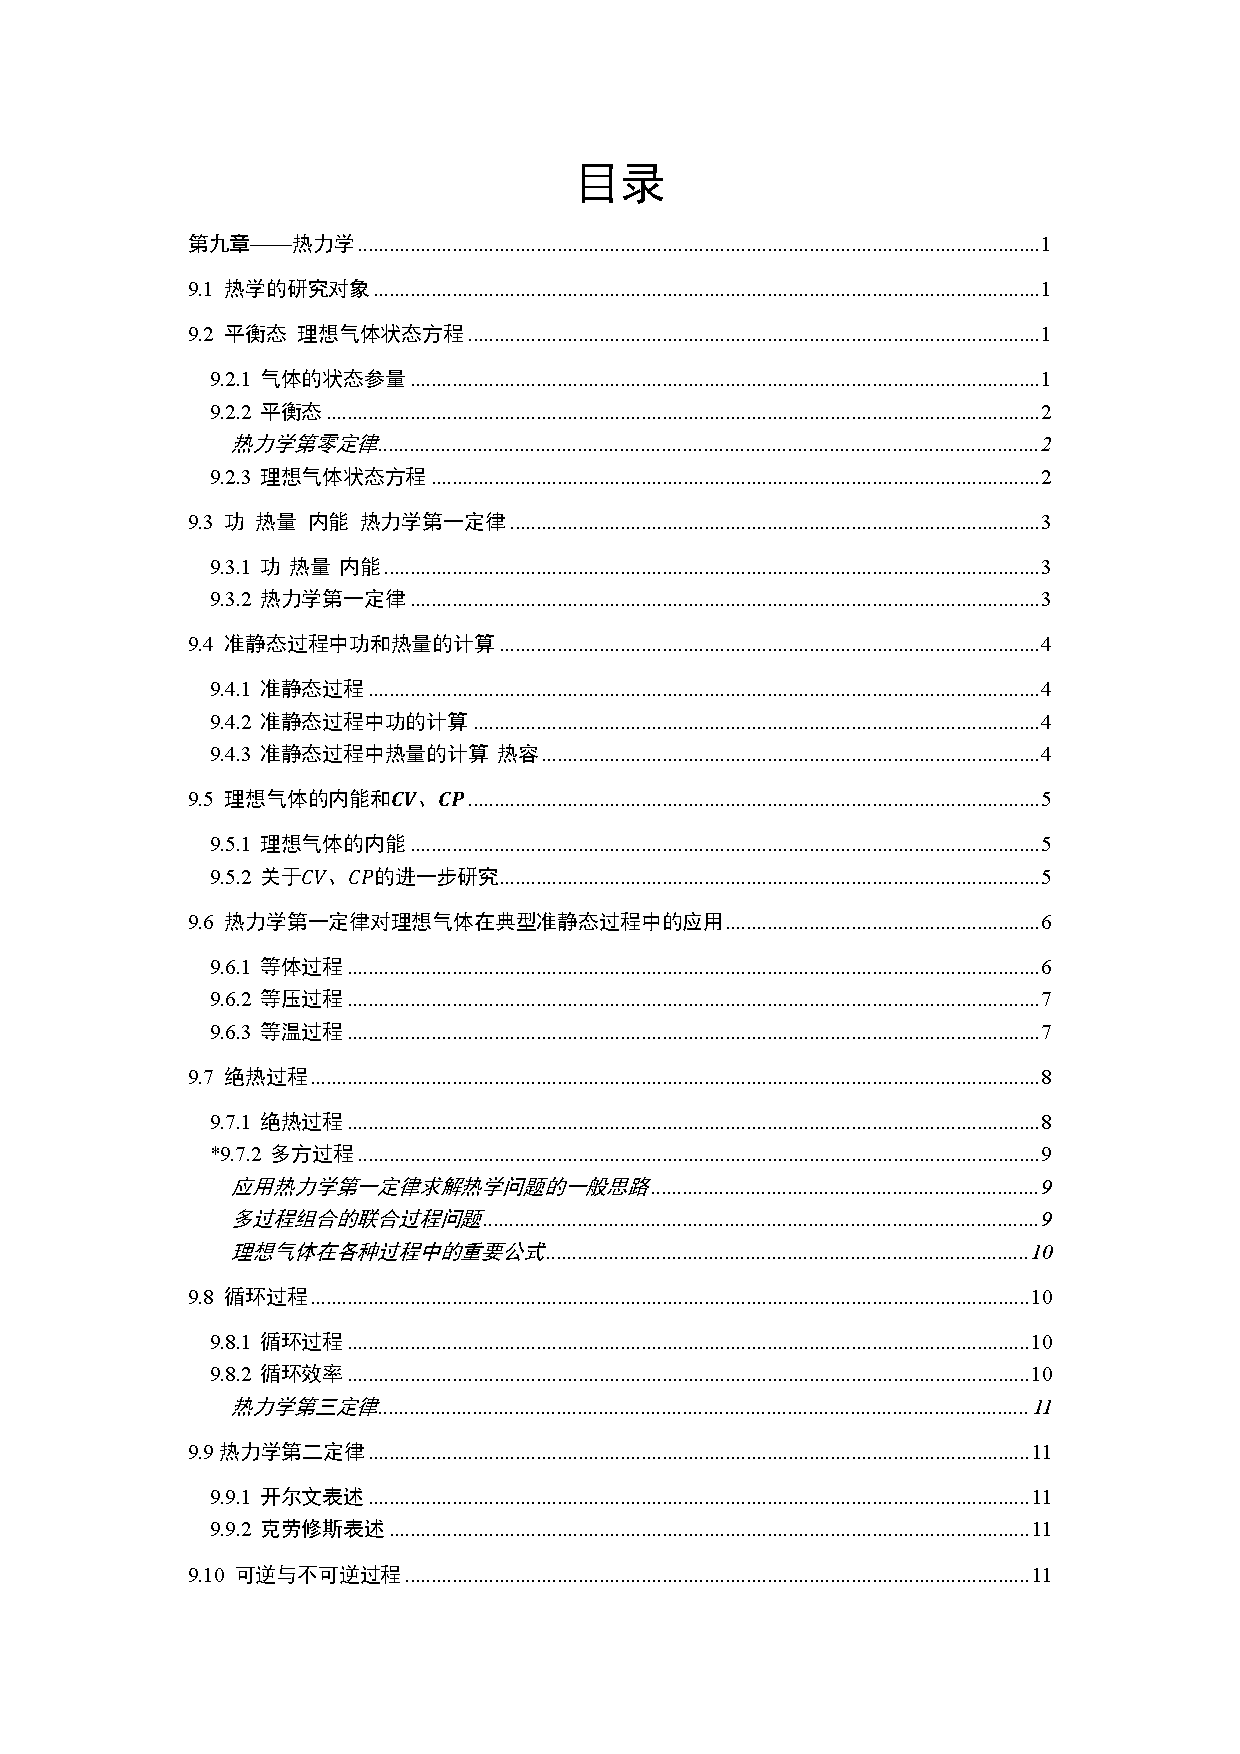
\includepdf[pagecommand = {\thispagestyle{empty}}, pages = - ]{toc.pdf}

\newpage
\setcounter{page}{1}
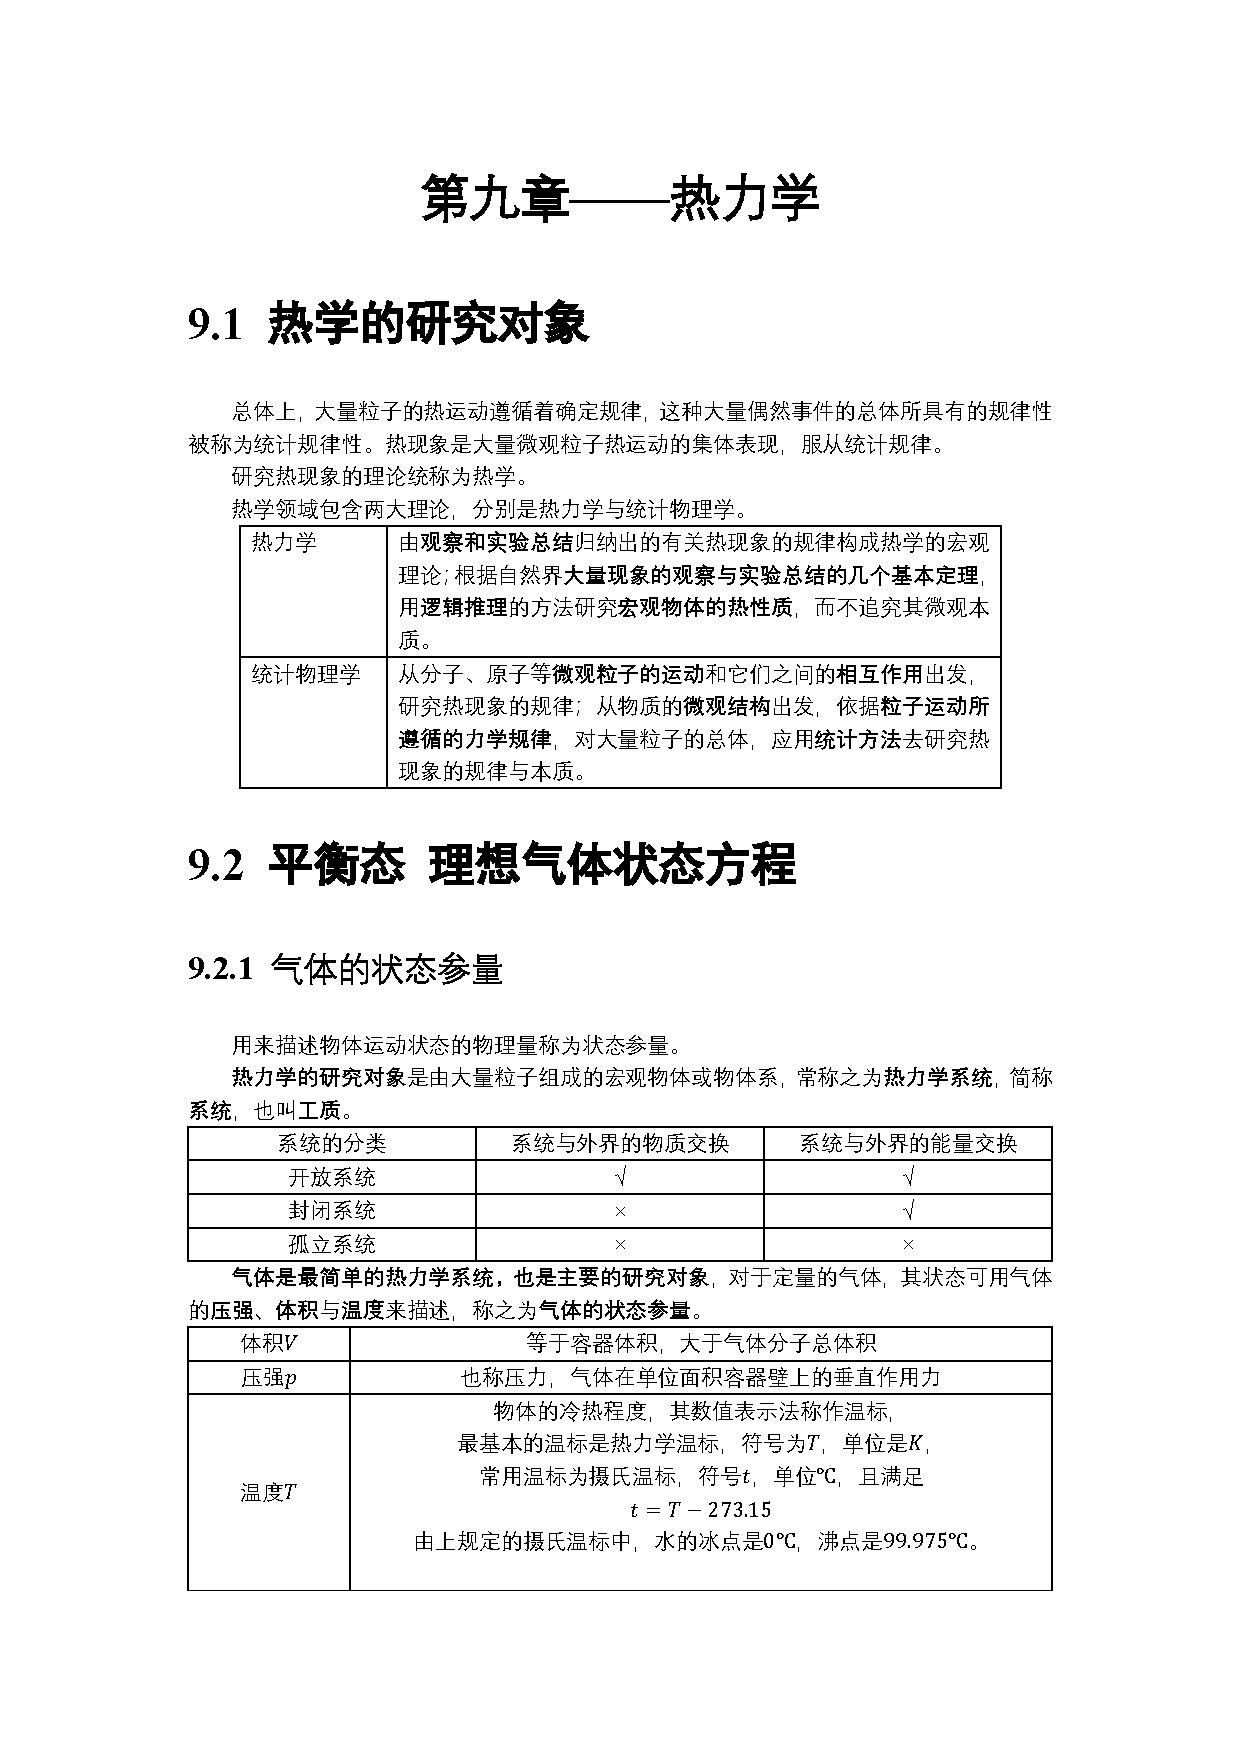
\includepdf[pages = - ]{content.pdf}


\end{document}